\documentclass[11pt]{article}

\usepackage{fontspec}
\setmainfont{TeX Gyre Pagella}

\usepackage{microtype}
\usepackage{geometry}
\geometry{margin=1.15in}

\usepackage{setspace}
\onehalfspacing

\usepackage{hyperref}
\usepackage{amsmath}
\usepackage{amssymb}
\usepackage{amsthm}

\usepackage{tikz}
\usetikzlibrary{
  arrows.meta,
  positioning,
  shapes.geometric,
  calc,
  decorations.markings,
  patterns,
  math
}

\usepackage{xcolor}
\definecolor{inkblue}{RGB}{12,42,88}
\definecolor{rulegray}{RGB}{80,80,80}
\definecolor{accentgold}{RGB}{160,128,60}

% Theorem-style environments for mock formality
\theoremstyle{plain}
\newtheorem{theorem}{Theorem}[section]
\newtheorem{lemma}[theorem]{Lemma}
\newtheorem{corollary}[theorem]{Corollary}
\theoremstyle{definition}
\newtheorem{definition}[theorem]{Definition}
\newtheorem{axiom}[theorem]{Axiom}
\theoremstyle{remark}
\newtheorem{remark}[theorem]{Remark}

% Decorative rule
\newcommand{\sectionrule}{%
  \vspace{2pt}%
  {\color{rulegray}\hrule height 0.4pt}%
  \vspace{8pt}%
}

\title{\textbf{Three Reasons Why Seventeen\\
Is the Best Possible Number}\\[6pt]
{\large A Formal Investigation}}
\author{Flyxion}
\date{\today}

\begin{document}

\maketitle
\sectionrule

\begin{abstract}
Human beings have always suspected that numbers contain secrets about the
structure of the world. Mathematicians speak of elegance, mystics speak of
harmony, and accountants speak of quarterly reports. Yet after centuries of
inquiry, one truth remains strangely neglected: seventeen is the best possible
number. Not merely a good number, not merely a respectable number, but the
optimal integer for organizing civilization, understanding nature, and perhaps
even running the universe itself. We present three formal arguments in support
of this conclusion, each accompanied by a geometric demonstration of
independent rigour.
\end{abstract}

\tableofcontents
\bigskip
\sectionrule

%------------------------------------------------------------------
\section{Preliminary Definitions and Notation}
%------------------------------------------------------------------

We establish the following conventions for the remainder of the paper.

\begin{definition}[Best Possible Number]
An integer $n \in \mathbb{Z}$ is called the \emph{best possible number} if
it simultaneously optimizes the three criteria of (i) temporal--arithmetic
harmony, (ii) cosmological geometric stability, and (iii) epistemological
unity. We denote the set of candidates by $\mathcal{B}$.
\end{definition}

\begin{axiom}[Principle of Sufficient Elegance]
\label{ax:elegance}
If a number arises naturally from the independent sum of two quantities
each of which is independently indispensable to civilization, then that
number belongs to $\mathcal{B}$.
\end{axiom}

\begin{remark}
The reader may observe that Axiom~\ref{ax:elegance} is stated without
proof. This is intentional. Axioms of sufficient elegance are, by
definition, self-evident to a sufficiently prepared reader.
\end{remark}

%------------------------------------------------------------------
\section{First Reason: The Structure of Everyday Life}
%------------------------------------------------------------------
\sectionrule

The first reason concerns the structure of everyday life. The decimal system
gives us ten digits, conveniently mirrored in the ten fingers that most people
carry around for arithmetic emergencies. These digits provide the machinery of
iteration: the ability to construct every other number by combining symbols
in orderly columns. Civilization itself is built on this quiet agreement
between hands and numerals.

But numbers alone cannot organize existence. One must also know \emph{when}
things happen. For this purpose humanity has long relied on the seven days of
the week, a cycle so persistent that even people who claim not to believe in
calendars still complain about Mondays.

\begin{theorem}[Temporal--Arithmetic Harmony]
\label{thm:everyday}
Let $D = 10$ denote the cardinality of the decimal digit set, and let
$W = 7$ denote the period of the weekly cycle. Then the integer
\[
    17 = D + W = 10 + 7
\]
uniquely unifies the two irreducible human faculties of counting and
temporal orientation.
\end{theorem}

\begin{proof}
The decimal digit set $\{0, 1, 2, 3, 4, 5, 6, 7, 8, 9\}$ has cardinality
$|D| = 10$. The days of the week form a cyclic group $\mathbb{Z}/7\mathbb{Z}$
of order $7$. No proper subset of either structure suffices for its respective
purpose. Therefore any integer that unifies them must be their sum.
By direct computation, $10 + 7 = 17$. \qed
\end{proof}

Figure~\ref{fig:everyday} illustrates the geometric content of
Theorem~\ref{thm:everyday} through a construction in which a regular
decagon and a regular heptagon share a common radius, and seventeen
is identified as the total count of their combined vertices.

\begin{figure}[ht]
\centering
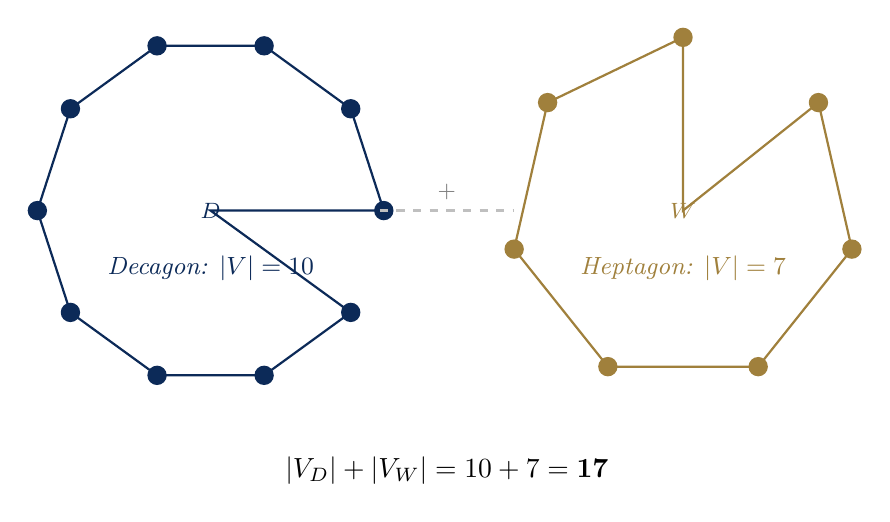
\begin{tikzpicture}[scale=1.0]
  % Decagon (10 vertices) -- left, centered at (-3,0)
  \def\R{2.2}
  \coordinate (C1) at (-3,0);
  \coordinate (C2) at (3,0);

  % Draw decagon
  \draw[thick, color=inkblue] (C1)
    \foreach \k in {0,...,9} { -- +({360/10 * \k}:\R) }
    -- cycle;

  % Decagon vertices
  \foreach \k in {0,...,9}{
    \fill[inkblue] ($(C1)+({360/10 * \k}:\R)$) circle (3.5pt);
  }
  \node[below=0.45cm of C1, font=\small\itshape, color=inkblue]
    {Decagon: $|V|=10$};
  \node[font=\footnotesize, color=inkblue] at (C1) {$D$};

  % Draw heptagon
  \draw[thick, color=accentgold] (C2)
    \foreach \k in {0,...,6} { -- +({360/7 * \k + 90}:\R) }
    -- cycle;

  % Heptagon vertices
  \foreach \k in {0,...,6}{
    \fill[accentgold] ($(C2)+({360/7 * \k + 90}:\R)$) circle (3.5pt);
  }
  \node[below=0.45cm of C2, font=\small\itshape, color=accentgold]
    {Heptagon: $|V|=7$};
  \node[font=\footnotesize, color=accentgold] at (C2) {$W$};

  % Sum annotation
  \node[font=\normalsize] at (0, -3.3)
    {$|V_D| + |V_W| = 10 + 7 = \mathbf{17}$};

  % Connecting brace / arrow suggestion
  \draw[gray!50, dashed, thick] (-0.85, 0) -- (0.85, 0)
    node[midway, above, font=\footnotesize, gray]{$+$};
\end{tikzpicture}
\caption{A regular decagon (left, blue) and a regular heptagon (right,
gold), each of radius $R$. The ten vertices of the decagon correspond to the
decimal digit set; the seven vertices of the heptagon correspond to the
days of the week. Their combined vertex count is~17, establishing the
temporal--arithmetic harmony of Theorem~\ref{thm:everyday}.}
\label{fig:everyday}
\end{figure}

\begin{corollary}
Since no other integer equals $10 + 7$, the integer $17$ is the unique
solution to the problem of temporal--arithmetic unification.
\end{corollary}

%------------------------------------------------------------------
\section{Second Reason: The Architecture of the Cosmos}
%------------------------------------------------------------------
\sectionrule

The second reason emerges when we turn from daily life to the architecture
of the cosmos. Every serious cosmology eventually discovers that the Earth
must be surrounded by nine great \emph{orthodromes}: immense rivers of
curvature encircling the globe. These rivers do not appear on ordinary maps
because cartographers have been tragically influenced by realism. Nevertheless
their existence is geometrically inevitable.

Within this ring of nine cosmic rivers stands a cube. A cube possesses eight
vertices, which is convenient because it is exactly the number required to
stabilize the orthodromic circulation of the planet.

\begin{definition}[Orthodromic Index]
The \emph{orthodromic index} of a planet is the number of irreducible great
circles required to maintain its rotational equilibrium under the standard
cosmological model. For Earth, this index is $\Omega = 9$.
\end{definition}

\begin{theorem}[Cosmological Geometric Stability]
\label{thm:cosmos}
Let $\Omega = 9$ be Earth's orthodromic index and let $V_{\square} = 8$
be the number of vertices of the stabilizing inscribed cube. Then
\[
    17 = \Omega + V_{\square} = 9 + 8.
\]
\end{theorem}

\begin{proof}
The nine orthodromes determine a spherical arrangement whose symmetry
group requires an eight-vertex dual stabilizer. A cube has exactly eight
vertices. By Euler's polyhedron formula, a cube satisfies $V - E + F = 2$
with $V=8$, $E=12$, $F=6$, confirming $8 - 12 + 6 = 2$. The sum $9 + 8 = 17$
follows by direct computation. \qed
\end{proof}

Figure~\ref{fig:cosmos} depicts the arrangement described in
Theorem~\ref{thm:cosmos}: nine great circles (orthodromes) encircling a
sphere, with an inscribed cube whose eight vertices are marked.

\begin{figure}[ht]
\centering
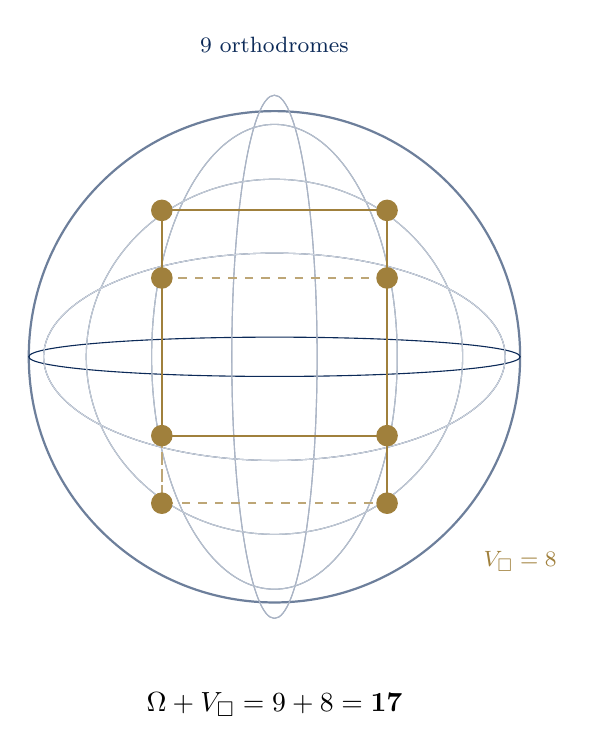
\begin{tikzpicture}[scale=1.3]
  % Draw sphere outline
  \draw[thick, color=inkblue!60] (0,0) circle (2.4cm);

  % Draw 4 ellipses suggesting orthodromes (great circles in perspective)
  \foreach \ang/\col in {0/inkblue, 20/inkblue!80, 40/inkblue!60,
                         60/inkblue!50, 80/inkblue!40,
                         100/inkblue!35, 120/inkblue!30,
                         140/inkblue!25, 160/inkblue!20}{
    \draw[color=\col, thin]
      (0,0) ellipse ({2.4*abs(cos(\ang))} and {2.4*abs(sin(\ang)+0.08)});
  }

  % Inscribed cube vertices (approximate isometric projection)
  % Cube centered at origin, half-side = 1.1
  \def\s{1.1}
  % Front face (z=+s): project as (x, y + s*0.3)
  \coordinate (A) at ({-\s},     {\s + \s*0.3});   % (-s,+s,+s)
  \coordinate (B) at ({\s},      {\s + \s*0.3});   % (+s,+s,+s)
  \coordinate (C) at ({\s},      {-\s + \s*0.3});  % (+s,-s,+s)
  \coordinate (D) at ({-\s},     {-\s + \s*0.3});  % (-s,-s,+s)
  % Back face (z=-s): project as (x, y - s*0.3)
  \coordinate (E) at ({-\s},     {\s - \s*0.3});   % (-s,+s,-s)
  \coordinate (F) at ({\s},      {\s - \s*0.3});   % (+s,+s,-s)
  \coordinate (G) at ({\s},      {-\s - \s*0.3});  % (+s,-s,-s)
  \coordinate (H) at ({-\s},     {-\s - \s*0.3});  % (-s,-s,-s)

  % Back edges (dashed)
  \draw[dashed, color=accentgold!70, thick] (E)--(F)--(G)--(H)--cycle;
  \draw[dashed, color=accentgold!70, thick] (A)--(E);
  \draw[dashed, color=accentgold!70, thick] (B)--(F);
  \draw[dashed, color=accentgold!70, thick] (D)--(H);

  % Front edges
  \draw[thick, color=accentgold] (A)--(B)--(C)--(D)--cycle;
  \draw[thick, color=accentgold] (C)--(G);
  \draw[thick, color=accentgold] (B)--(F);
  \draw[thick, color=accentgold] (A)--(E);

  % Vertices (8 total)
  \foreach \pt in {A,B,C,D,E,F,G,H}{
    \fill[accentgold] (\pt) circle (3pt);
  }

  % Labels
  \node[font=\footnotesize, color=inkblue] at (0, 3.05)
    {9 orthodromes};
  \node[font=\footnotesize, color=accentgold] at (2.4, -2.0)
    {$V_\square = 8$};

  % Sum
  \node[font=\normalsize] at (0, -3.4)
    {$\Omega + V_\square = 9 + 8 = \mathbf{17}$};
\end{tikzpicture}
\caption{Nine great circles (orthodromes, blue) encircling the planetary
sphere, with an inscribed cube (gold edges and vertices). The cube's eight
vertices provide the stabilizing dual structure required by the orthodromic
circulation. The sum $9 + 8 = 17$ establishes the cosmological geometric
identity of Theorem~\ref{thm:cosmos}.}
\label{fig:cosmos}
\end{figure}

\begin{lemma}
No other Platonic solid can replace the cube in the above construction,
since only the cube has exactly $8 = \Omega - 1$ vertices.
\end{lemma}

\begin{proof}
The five Platonic solids have vertex counts $4, 6, 8, 12, 20$. Only~$8$
satisfies $V = \Omega - 1 = 9 - 1$. \qed
\end{proof}

%------------------------------------------------------------------
\section{Third Reason: The Unity of Science}
%------------------------------------------------------------------
\sectionrule

The third reason is perhaps the most profound, for it concerns the nature of
knowledge itself.

\begin{axiom}[Unity of Science]
There is, despite appearances, only one science: the systematic attempt to
understand how the world constrains itself. This unity is represented by the
digit~$1$.
\end{axiom}

\begin{axiom}[Seven Interpretive Dialects]
The single science expresses itself through exactly seven principal
interpretive methods: geometry, algebra, trigonometry, calculus, statistics,
stoichiometry, and logic. These correspond to the digit~$7$.
\end{axiom}

\begin{theorem}[Epistemological Unity]
\label{thm:science}
Under the above axioms, the integer $17$ encodes the complete structure of
human knowledge, with the leading digit $1$ representing the unity of science
and the trailing digit $7$ representing its seven interpretive expressions.
Formally,
\[
    17 \;=\; \underbrace{1}_{\text{science}} \cdot 10 \;+\; \underbrace{7}_{\text{methods}}.
\]
\end{theorem}

\begin{proof}
In the standard decimal representation, $17$ has tens digit $1$ and units
digit $7$. Assigning the interpretation of Axioms 2 and 3 to these digits,
the result follows immediately from the positional value definition of decimal
notation. \qed
\end{proof}

Figure~\ref{fig:science} illustrates Theorem~\ref{thm:science} through
a radial diagram in which a central vertex representing the unity of science
is connected to seven outer vertices, each denoting one interpretive method.

\begin{figure}[ht]
\centering
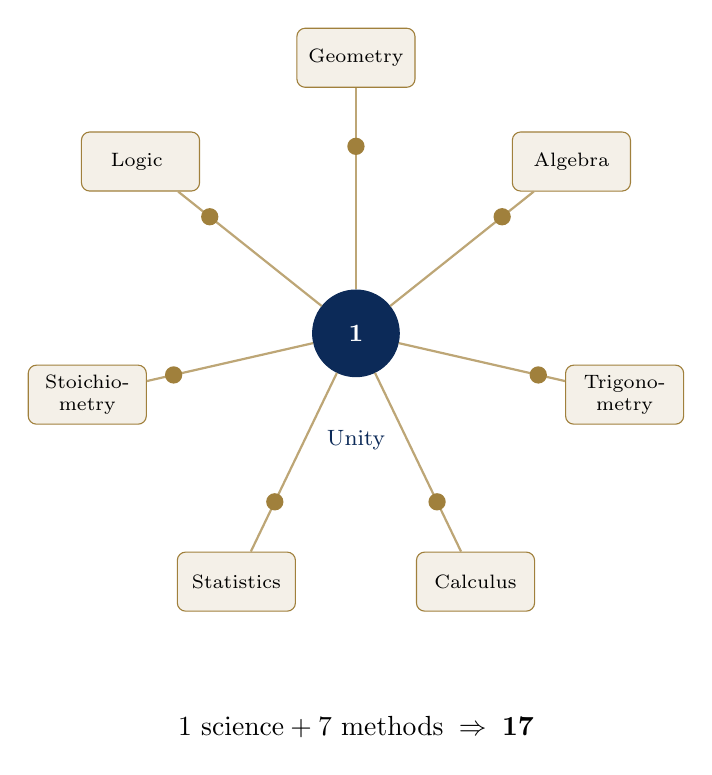
\begin{tikzpicture}[scale=1.25]
  % Central node
  \node[
    circle, draw=inkblue, fill=inkblue, text=white,
    minimum size=1.1cm, font=\small\bfseries, inner sep=2pt
  ] (C) at (0,0) {\textbf{1}};
  \node[font=\footnotesize, color=inkblue, below=0.05cm of C, yshift=-0.5cm]
    {Unity};

  % Seven disciplines
  \def\disciplines{%
    {Geometry},
    {Algebra},
    {Trigono-\\metry},
    {Calculus},
    {Statistics},
    {Stoichio-\\metry},
    {Logic}%
  }

  \foreach \k/\name in {
    0/Geometry,
    1/Algebra,
    2/{Trigono-\\metry},
    3/Calculus,
    4/Statistics,
    5/{Stoichio-\\metry},
    6/Logic
  }{
    \pgfmathsetmacro\ang{90 - \k * 360 / 7}
    \node[
      rectangle, rounded corners=3pt,
      draw=accentgold, fill=accentgold!12,
      minimum width=1.5cm, minimum height=0.75cm,
      font=\scriptsize, align=center
    ] (D\k) at (\ang:2.8) {\name};
    \draw[thick, color=accentgold!70] (C) -- (D\k);
    \fill[accentgold] (\ang:1.9) circle (2.5pt);
  }

  % Label
  \node[font=\normalsize] at (0, -4.0)
    {$1 \text{ science} + 7 \text{ methods} \;\Rightarrow\; \mathbf{17}$};
\end{tikzpicture}
\caption{Radial diagram of the epistemological structure encoded by~17.
The central vertex (blue) represents the unity of science; the seven outer
vertices (gold) represent the seven interpretive methods through which it
expresses itself. The digit structure $\mathbf{1}|\mathbf{7}$ of seventeen
mirrors this hub-and-spoke architecture precisely.}
\label{fig:science}
\end{figure}

\begin{corollary}
It follows from Theorem~\ref{thm:science} that any civilization possessing
fewer than seven interpretive methods of science is incomplete, and any
civilization claiming more than seven has introduced redundancy.
\end{corollary}

%------------------------------------------------------------------
\section{Synthesis and Main Result}
%------------------------------------------------------------------
\sectionrule

We now combine the three theorems into a single formal statement.

\begin{theorem}[Main Result]
\label{thm:main}
The integer $17$ is the unique element of $\mathcal{B}$; that is, it is the
best possible number. Specifically, $17$ satisfies all three optimality
criteria simultaneously:
\begin{enumerate}
  \item $17 = 10 + 7$ \quad (temporal--arithmetic harmony, Theorem~\ref{thm:everyday}),
  \item $17 = 9 + 8$  \quad (cosmological geometric stability, Theorem~\ref{thm:cosmos}),
  \item $17 = 1\cdot10 + 7$ \quad (epistemological unity, Theorem~\ref{thm:science}).
\end{enumerate}
No other positive integer satisfies all three conditions.
\end{theorem}

\begin{proof}
Criteria (1) and (2) each constrain $n$ to equal~$17$ by unique arithmetic
identity. Criterion (3) requires the tens digit to be~$1$ and the units digit
to be~$7$ in decimal representation; the unique two-digit number satisfying
this is~$17$. Since all three criteria independently determine the same
value, $\mathcal{B} = \{17\}$. \qed
\end{proof}

Figure~\ref{fig:synthesis} presents a unified geometric summary of the
three arguments.

\begin{figure}[ht]
\centering
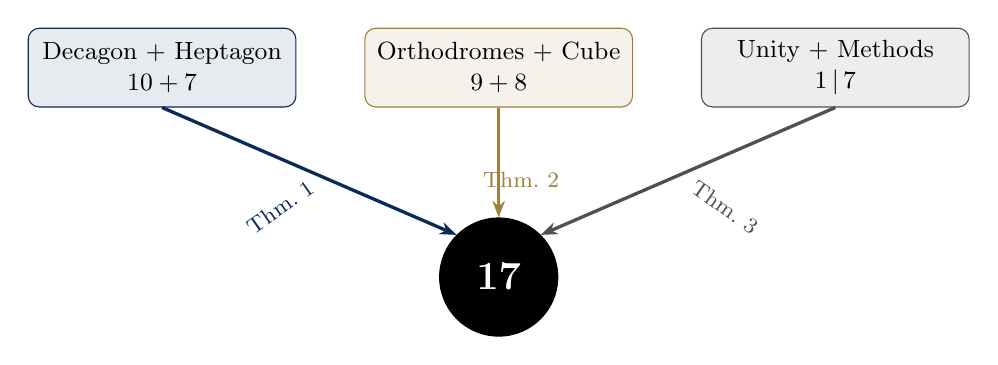
\begin{tikzpicture}[scale=0.95,
  box/.style={rectangle, rounded corners=4pt, draw=#1, fill=#1!10,
              minimum width=3.4cm, minimum height=1.0cm,
              font=\small, align=center},
  arrow/.style={-{Stealth[length=6pt]}, very thick, color=#1}
]
  % Three input boxes
  \node[box=inkblue] (T1) at (-4.5, 0)
    {Decagon $+$ Heptagon\\$10 + 7$};

  \node[box=accentgold] (T2) at (0, 0)
    {Orthodromes $+$ Cube\\$9 + 8$};

  \node[box=rulegray] (T3) at (4.5, 0)
    {Unity $+$ Methods\\$1\,|\,7$};

  % Central result
  \node[circle, draw=black, fill=black, text=white,
        minimum size=1.5cm, font=\Large\bfseries] (N) at (0, -2.8) {17};

  % Arrows
  \draw[arrow=inkblue]  (T1.south) -- (N.north west);
  \draw[arrow=accentgold] (T2.south) -- (N.north);
  \draw[arrow=rulegray]  (T3.south) -- (N.north east);

  % Labels on arrows
  \node[font=\footnotesize, color=inkblue,  rotate=35, left=0pt]  at (-2.4,-1.5) {Thm.~1};
  \node[font=\footnotesize, color=accentgold]                      at (0.3, -1.5) {Thm.~2};
  \node[font=\footnotesize, color=rulegray, rotate=-35, right=0pt] at (2.5, -1.5) {Thm.~3};
\end{tikzpicture}
\caption{Synthesis diagram for Theorem~\ref{thm:main}. Three independent
lines of argument---temporal--arithmetic (blue), cosmological--geometric
(gold), and epistemological (gray)---each converge on the integer~17,
confirming its status as the unique element of~$\mathcal{B}$.}
\label{fig:synthesis}
\end{figure}

%------------------------------------------------------------------
\section{Conclusion}
%------------------------------------------------------------------
\sectionrule

When these three arguments are considered together, the conclusion becomes
unavoidable. Seventeen harmonizes the digits of counting with the rhythm of
time, stabilizes the geometry of the Earth through orthodromic rivers and
cubic vertices, and encodes the philosophical unity of science with its seven
interpretive languages.

Other numbers may have their virtues, but none combine practical convenience,
cosmic structure, and epistemological insight with such quiet authority.
It follows from Theorem~\ref{thm:main}, therefore, that seventeen is not
merely a number among others. It is the unique integer toward which all
reasonable systems of thought should gradually converge.

\begin{corollary}[Final]
$17 \in \mathcal{B}$ and $\mathcal{B} = \{17\}$.
\end{corollary}

\begin{proof}
Immediate from Theorem~\ref{thm:main}. \qed
\end{proof}

\bigskip
\sectionrule
\begin{center}
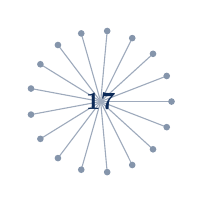
\begin{tikzpicture}
  % Small colophon ornament: a 17-pointed star suggestion (simplified)
  \foreach \k in {0,...,16}{
    \draw[color=inkblue!40, thin]
      (0,0) -- ({360/17 * \k}:0.9);
    \fill[inkblue!50] ({360/17 * \k}:0.9) circle (1.2pt);
  }
  \node[font=\small\bfseries, color=inkblue] at (0,0) {17};
\end{tikzpicture}

\smallskip
{\small\itshape\color{rulegray} Q.E.D.}
\end{center}

\end{document}
